\section{Automatyzacja a branża IT}
\subsection{Charakteryzacja branży IT}
W 2001 roku doszło do jednej z bardziej znaczących publikacji dla szerokopojętego biznesu IT. W roku tym został opublikowany \textit{Manifesto for Agile Software Development} autorstwa między innymi Kenta Becka, Roberta C. Martina oraz Martina Fowlera. Manifest ten opisywał rewolucyjne jak na tamte czasy praktyki \cite{AgileManifesto}:
\begin{itemize}
    \item Satysfakcja klienta dzięki wczesnemu i ciągłemu dostarczaniu oprogramowania.
    \item Zmiany wymagań mile widziane nawet na późnym etapie programowania.
    \item Dostarczanie działającej wersji oprogramowanie często (bardziej tygodnie niż miesiące).
    \item Bliska kooperacja między programistami a ludziami zajmującymi się biznesem
    \item Projekty powstają wokół zmotywowanych osób, którym należy ufać.
    \item Komunikacja w cztery oczy jest najlepszą formą komunikacji
    \item Działający produkt jest najlepszym wskaźnikiem postępu prac.
    \item Zrównoważony rozwój, pozwalający na utrzymania stałego tempa.
    \item Ciągła dbałość o doskonałość techniczną i dobry design.
    \item Prostota - sztuka projektowania systemu bez dużej komplikacji systemu.
    \item Najlepsze architektury, wymagania i designy powstają dzięki samoorganizującym się zespołom
    \item Zespół regularnie zastanawia się, jak zwiększyć skuteczność, i odpowiednio się dostosowuje. 
\end{itemize}
Propozycje przedstawione przez autorów manifestu były dużą zmianą w stosunku do podejścia które było używane powszechnie w tamtych czasach.
\par
W latach 80 oraz 90 powszechnie stosowaną techniką była metodologia Waterfall zobrazowana na Rysunku \ref{fig:waterfall}.
\begin{figure}[htbp]
    \centering
    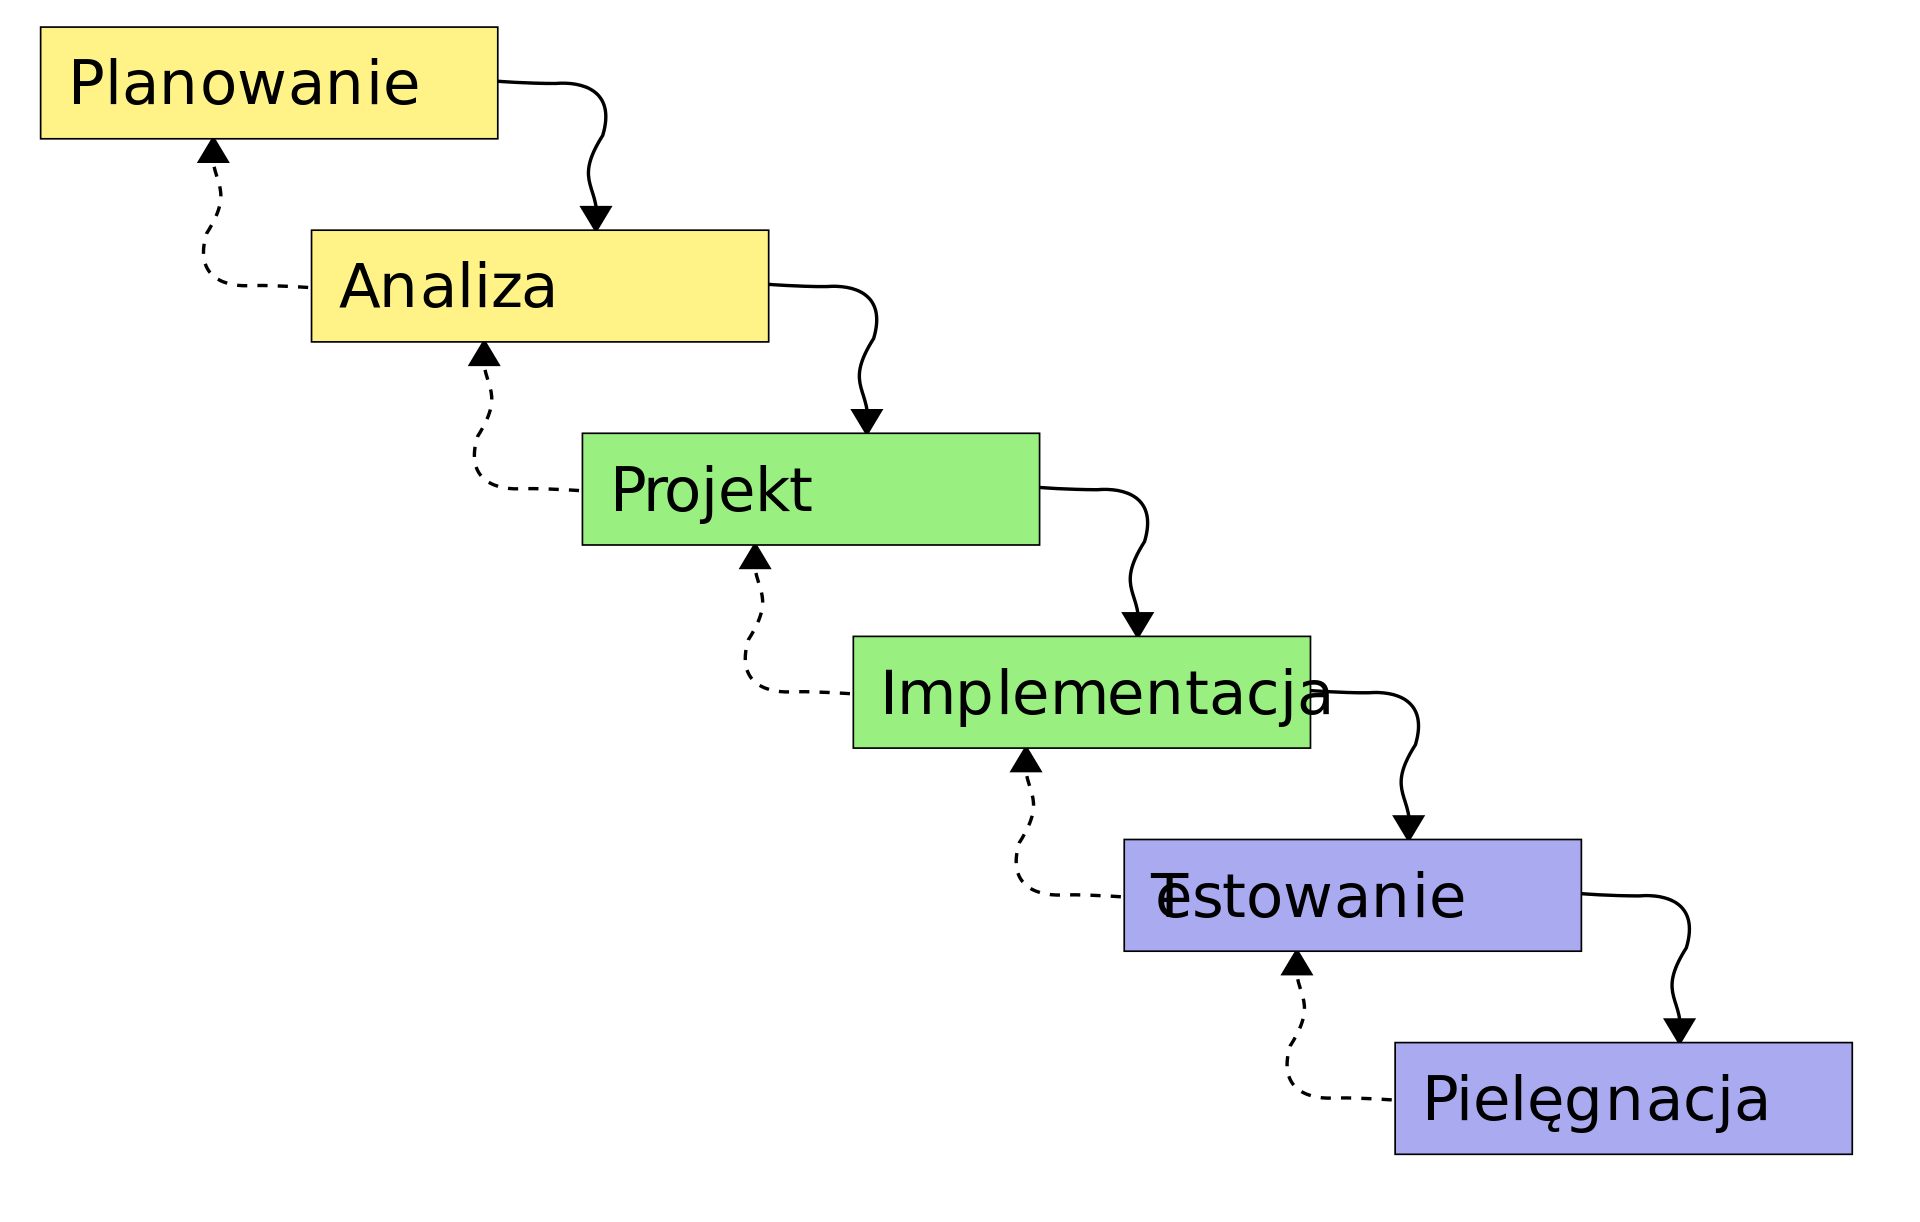
\includegraphics[width=10cm]{waterfall.png}
    \caption{Metodologia Waterfall}
    \label{fig:waterfall}
\end{figure}
Poszczególne etapy projektowe były wykonywane tylko raz podczas procesu tworzenia oprogramowania. Z tego faktu wszelakie zmiany na późniejszym etapie projektowym były trudne w realizacji. Konkurencja na rynku oprogramowania komputerowego była na tyle niewielka, że producenci oprogramowania nie musieli przejmować się zanadto uwagami od użytkowników - to sprawiało, że Waterfall spełniał swoje zadania. 
\par
Pierwsze dziesięciolecie XXI wieku spopularyzowało jedno z największych osiągnięć ludzkości - Internet. Nowa rzeczywistość w której ludzkość coraz więcej czasu spędza przed urządzeniami elektronicznymi postawiła przez twórcami oprogramowania nowe wymagania. Dodatkowo coraz większe grono przedsiębiorców zaczyna dostrzegać w produkcji oprogramowania zyski. Użytkownicy zaczynają coraz bardziej spoglądać na przyjemny dla oka wygląd oprogramowania oraz jego prostotę. Metodyka zaproponowana przez autorów manifestu Agile zdaje się świetnie wpisywać w wizję tworzenia oprogramowania na miarę XXI wieku.
\par
Jedną z bardziej znanych implementacji Agile jest metodologia o nazwie Scrum.
\begin{figure}[htbp]
    \centering
    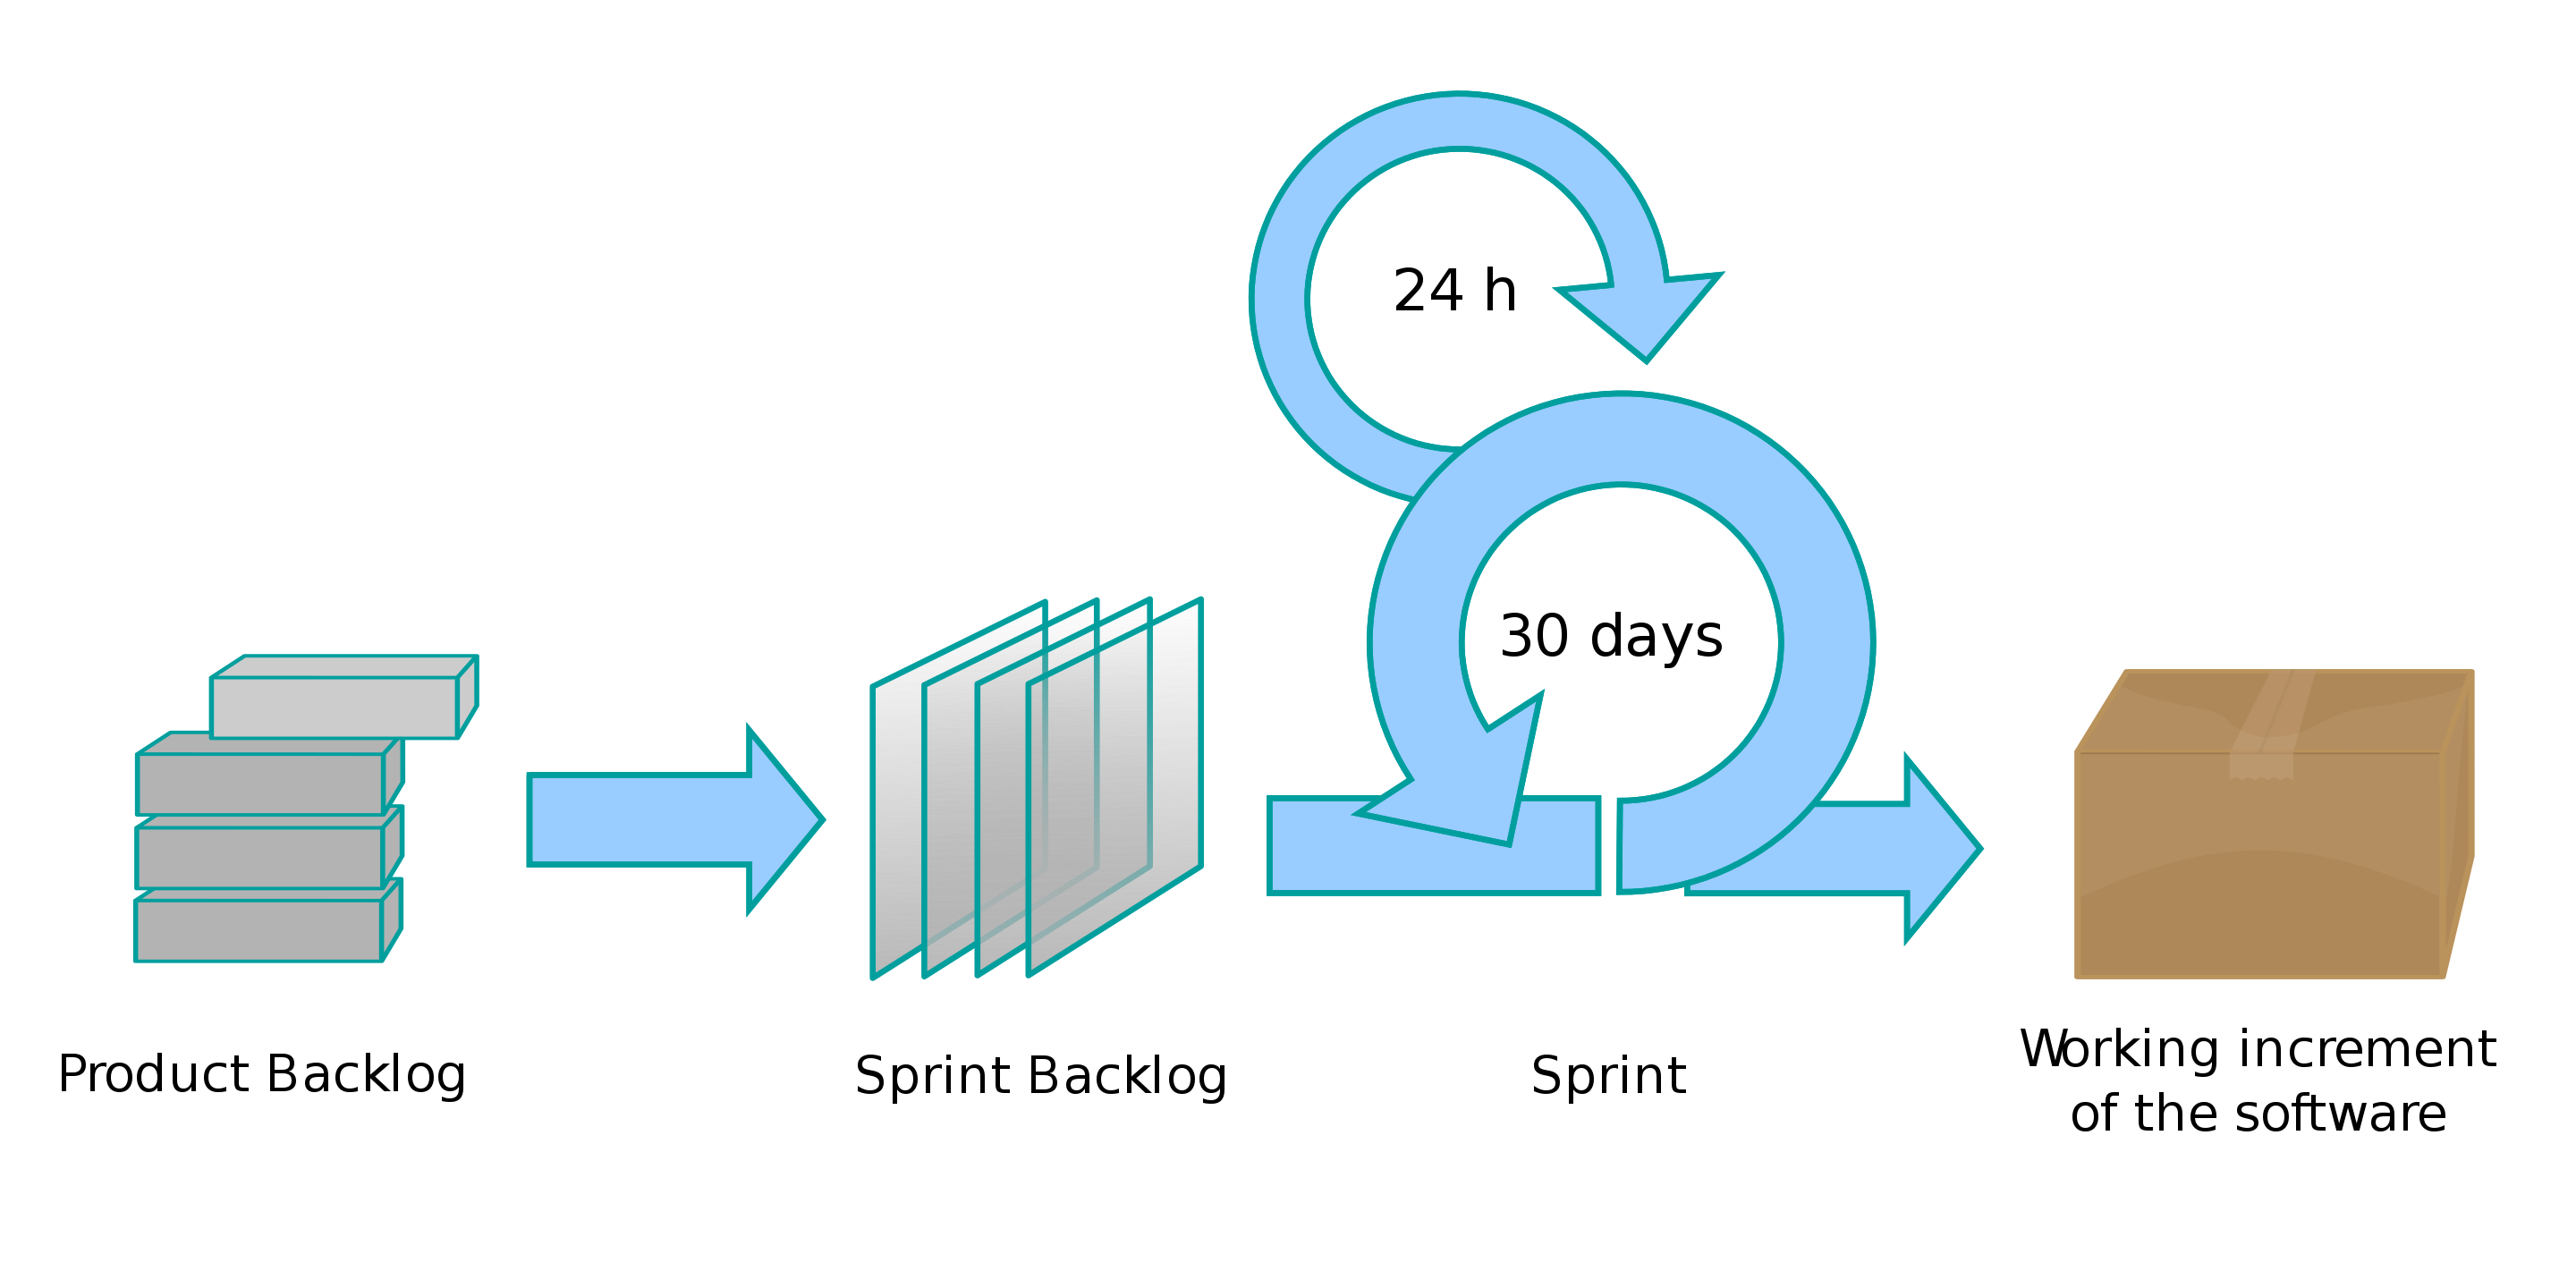
\includegraphics[width=10cm]{scrum.png}
    \caption{Framework Scrum}
    \label{fig:scrum}
\end{figure}
Zakłada się w niej, że oprogramowanie powstaje w procesie kolejnych inkrementacji. Każda iteracja jest nazywana sprintem. Sprint ma z góry zdefiniowane ramy czasowe w których będzie on trwał. Na podstawie różnych czynników biznesowych opiekun projektu decyduje które zadania powinny trafić do danego sprintu, a które są mniej priorytetowe i mogą pozostać w tzw. backlogu. Efektem końcowym danego sprintu jest działający produkt, który jest wzbogacony o rzeczy dodane podczas trwania sprintu. Scrum sam w sobie nie narzuca ile powinien trwać dany sprint, czy też jaki system powinien być stosowany do śledzenia zadań. Wszystko zależy od preferencji danego zespołu programistycznego. Integralną częścią każdego sprintu jest retrospektywa. Na tym spotkaniu zespół dyskutuje jakie zmiany należy dokonać w procesie by uefektywnić pracę. Dzięki elastycznemu podejściu i możliwości ulepszania procesu Scrum wydaje się być dobrym rozwiązaniem dla zespołów które wypuszczają oprogramowanie regularnie oraz zmieniają je na podstawie opinii użytkowników.
\subsection{Agile a automatyzacja}
Spełnienie wymagań wymienionych w manifeście Agile wydaje się być trudne w kontekście częstego wypuszczania działającej wersji. Oczekuje się tego by regularnie zespół deweloperski publikował działającą wersję podglądową oprogramowania dla osób nietechnicznych. Problem ten można rozwiązać na conajmniej dwa sposoby:
\begin{itemize}
    \item Manualny - Członek zespołu deweloperskiego regularnie według wymagań zajmuje się budowaniem wersji podglądowej oraz udostępnia ją osobom zainteresowanym
    \item Automatyczny - Zespół deweloperski ustawia automatyczne procesy które na serwerze budującym tworzą wersję podglądową aplikacji oraz publikują ją dla osób zainteresowanych
\end{itemize}
Proces automatyczny jest preferowanym sposobem publikacji oprogramowania. Ma on kilka zalet nad sposobem manualnym. Nie tracimy czasu specjalisty który musiałby poświęcić go na zbudowanie i publikację aplikacji. Drugą zaletą jest fakt, że serwer za każdym razem robi te same kroki podczas procesu budowania. Tym sposobem wykluczamy możliwość popełnienia błędu przez człowieka.
\par
Dobre praktyki związane z częstym budowaniem podglądowej wersji oprogramowania są określane jako DevOps. Len Bass, Ingo Weber oraz Liming Zhu w swojej książce \cite{DevOpsBook} określają DevOps jako zbiór praktyk których celem jest zmniejszenie czasu publikacji zmian na serwerze produkcyjnym przy jednoczesnej trosce o wysoką jakość. W praktyce często członkiem zespołu deweloperskiego jest tzw. DevOps. Jego zadaniem jest automatyzacja wszelakich procesów oraz często także utrzymanie środowiska produkcyjnego. Osoba na tym stanowisku powinna się cechować dobrą znajomością systemu operacyjnego który jest używany na serwerach produkcyjnych oraz deweloperskich. Ponadto powinna być zorientowana w różnych rozwiązaniach chmurowych które współcześnie są coraz częściej używane.
\subsection{Git - kamień milowy dla deweloperów}
Ciężko byłoby sobie wyobrazić obraz dzisiejszego przemysłu IT gdyby nie system kontroli wersji Git. Jego autorem jest Linus Torvalds. Torvalds stworzył go jako dodatkowy projekt który miał pomóc w pisaniu jądra Linuxa. Dzięki Git'owi każdy członek zespołu deweloperskiego ma dostęp do wspólnego repozytorium gdzie każdy może publikować swoje zmiany. Jedną z ważniejszych funkcji Git'a jest możliwość tworzenia własnych rozgałęzień kodu gdzie dany programista wysyła swoje zmiany. Dalej w procesie merge'owania jest możliwe połączenie zmian danego dewelopera z kodem innych programistów. Dzięki tej cesze Git nadaje się świetnie do wszelakich projektów programistycznych w których pracuje kilku programistów równolegle. Z biegiem lat Git stał się standardem.
\par
Opisać git workflow TODO!!
\par
W obecnych czasach popularne są rozwiązania SaaS takie jak GitHub, GitLab czy też BitBucket. Dzięki takiemu rozwiązaniu nie musimy się przejmować utrzymaniem własnego serwera Git, dodatkowo platformy SaaS zapewniają nam wszelakie aktualizacje które usprawniają system. Platformy takie jak GitHub zapewniają narzędzie które ułatwiają proces tworzenia oprogramowania. Narzędzie te są dopasowane by działać dobrze z naszym repozytorium. Przykładem takiego rozwiązania jest \textit{GitHub Pages}, jest to technologia która pozwala publikować stronę www na podstawie plików które są częścią repozytorium. Użytkownik definiuje na której gałęzi oraz w którym folderze znajdują się pliki z stroną internetową. Od tego momentu GitHub automatycznie stwarza nam stronę internetową dostępną pod subdomeną \textit{nazwauzytkownika.github.io}.
\subsection{Ciągła integracja}
\subsection{Ciągłe dostarczanie}
\subsection{Ciągłe dowożenie}
\subsection{Serwery automatyzujące PaaS kontra self-hosted}
\subsection{GitOps - czym jest?}